\documentclass{article}
% --- watermark (auto-inserted) ---
\usepackage{xcolor}
\usepackage{xfp}% \fpeval; in the kernel since 2022, harmless on older LaTeX
\usepackage{draftwatermark}
\newlength{\watermarkTextWidth}
\AddToHook{begindocument/end}{%
  \SetWatermarkText{\normalfont Generated by The Agentic Scientist}%
  \SetWatermarkFontSize{10pt}%
  \SetWatermarkLightness{0.85}%
  \settowidth{\watermarkTextWidth}{\normalfont\fontsize{10pt}{12pt}\selectfont Generated by The Agentic Scientist}%
  \edef\watermarkScale{\fpeval{0.8 * sqrt(\paperwidth**2 + \paperheight**2) / \watermarkTextWidth}}%
  \edef\watermarkAngle{\fpeval{atand(\paperheight/\paperwidth)}}%
  \SetWatermarkScale{\watermarkScale}%
  \SetWatermarkAngle{\watermarkAngle}%
}
% --- end watermark ---
 % For LaTeX2e
\usepackage{paper,times}

\usepackage{hyperref}
\usepackage{url}
\usepackage{graphicx}
\usepackage{booktabs}
\usepackage{amsmath,amssymb}

\newcommand{\IS}{\mathrm{IS}}
\newcommand{\theHat}{\hat\theta}

\title{Reporting Scores After Prompt Search: A Selection-Aware Posterior Interval from a Hierarchical Latent-Difficulty Model}
\iclrfinalcopy
\author{The Agentic Scientist}

\begin{document}
\maketitle

\begin{abstract}
Automatic prompt and pipeline search reuses one benchmark sample both to choose a configuration and to score it, so the reported score can overstate accuracy on fresh questions.
We measure this optimism in controlled worlds with known truth---synthetic latent-difficulty worlds and cached outcomes of Qwen2.5-0.5B-Instruct on MMLU-Pro under 24 prompt configurations, searched exhaustively or by successive halving---and test a searcher-agnostic remedy.
The naive best-of-search score overstates fresh-question accuracy by 0.037 on average (about 0.05 at 60 benchmark questions), and its nominal 90\% Wilson interval contains the fresh accuracy in only 71\% of replications.
The remedy fits an empirical-Bayes hierarchical logistic latent-difficulty model to the full search log and reports posterior quantiles.
In a sealed evaluation over eight seeds it lowers the mean 90\%-level interval score to 0.145, against 0.220 (naive), 0.197 (Bonferroni-widened Wilson) and 0.246 (question resampling), with coverage 0.929; the evaluator's qualification outcome is ``qualified''.
The gain is regime-dependent: the reporter only ties the naive interval under halving on real outcomes and at 600 questions, and ties resampling under exhaustive search; in those two real-outcome cases its coverage is 0.89 (halving, within seed noise of nominal) and 0.83 (600 questions, clearly below nominal).
The evidence covers one small model, one benchmark and a hand-set width calibration, and does not test effects on ranking decisions.
\end{abstract}
% @evidence[[paper_data.json#final.metric.mean_interval_score]]
% @evidence[[paper_data.json#final.metric.naive_baseline_score]]
% @evidence[[paper_data.json#final.metric.bonferroni_baseline_score]]
% @evidence[[paper_data.json#final.metric.resample_baseline_score]]
% @evidence[[paper_data.json#final.metric.coverage]]
% @evidence[[paper_data.json#final.metric.naive_signed_bias]]
% @evidence[[paper_data.json#final.qualification.outcome]]
% @evidence[[analysis/reconstructed_baselines.json#aggregate_primary.naive_cov]]
% @evidence[[analysis/final_per_case.json#cases.P5.naive_bias]]
% @evidence[[analysis/final_per_case.json#cases.P4.coverage]]
% @evidence[[analysis/final_per_case.json#cases.P6.coverage]]

\section{Introduction}
Prompt and pipeline optimizers such as DSPy and MIPRO search over instructions, demonstrations and multi-call structures on a benchmark sample \citep{Khattab2023DSPy,OpsahlOng2024MIPRO}, LLM-driven optimizers propose and rank candidate prompts by their score on a task sample \citep{Zhou2022APE,Yang2023OPRO}, and in practice the best configuration is often reported with the score it attained on the very sample used to select it. Configuration search is also cast as best-arm identification under a fixed evaluation budget \citep{Shi2024PromptBAI}. The reported number is the maximum, over many candidates, of noisy estimates, and the candidate that attains it was chosen \emph{because} its estimate was high. It is therefore a biased estimate of that candidate's accuracy on new questions, and the usual interval around it ignores the selection. This is the selection bias long documented for model selection, where the score used to pick among many candidates is an optimistic performance estimate \citep{Cawley2010Overfitting}. Whether comparisons and decisions built on such numbers are trustworthy depends on how large the gap is and on what controls it.

We ask two questions. \textbf{(Q1)} For a system whose configuration is chosen on a finite question set, how far is the reported score from its accuracy on fresh questions, what governs the gap, and does it threaten conclusions drawn from reported scores? \textbf{(Q2)} Can a better reporting rule be designed, and how should its reliability be tested?

Our answer to Q2 is a post-hoc \emph{reporter} that never touches the search: it receives only the evaluation log of (question, configuration, outcome) triples, the selected configuration and basic metadata, and returns a point estimate and a 90\% interval for the selected configuration's fresh-question accuracy. The reporter fits a hierarchical logistic latent-difficulty model with empirical-Bayes variance components (EB-IRT). Because both searchers we study choose using only observed outcomes, selection is ignorable for the likelihood, so one fitting routine serves exhaustive search and successive halving. Shrinkage of configuration effects addresses the winner's curse directly; the interval is formed from posterior quantiles, which are the optimal report under the interval score \citep{Gneiting2007Scoring}.

We test reliability with an evaluator that owns the data-generating worlds, the searchers and the truth, so that coverage and interval score are measured against known fresh-question accuracy. Worlds are synthetic latent-difficulty worlds and cached real outcomes of Qwen2.5-0.5B-Instruct \citep{Qwen2024Qwen25} on MMLU-Pro \citep{Wang2024MMLUPro} under 24 prompt configurations, plus three negative controls.

\textbf{Contributions.} (i) A quantification of the optimism of best-of-search reporting and of the coverage of its Wilson interval across question budget, world and searcher (Section~\ref{sec:gap}). (ii) A searcher-agnostic EB-IRT reporter with a reimplementable specification (Section~\ref{sec:method}). (iii) A controlled evaluation protocol with known truth, null and constant-world controls, and seed-level uncertainty, applied to four reporters in a sealed final run (Sections~\ref{sec:protocol}--\ref{sec:controls}). (iv) A candid map of where the reporter fails to improve on simpler reporters: real-outcome halving, large question budgets, and exhaustive search where question resampling is as good.

\textbf{Scope.} The worlds, searchers, baseline reporters and scoring were supplied as a fixed evaluation harness, and the real-outcome tensors were produced beforehand by the task authors; this study ran neither LLM inference nor a DSPy/MIPRO search. Claims are conditional on one 0.5B model, one benchmark, one 24-configuration prompt family and two searchers. We do not test whether the optimism changes the \emph{ranking} of systems (Section~\ref{sec:limits}).

\begin{figure}[t]
\centering
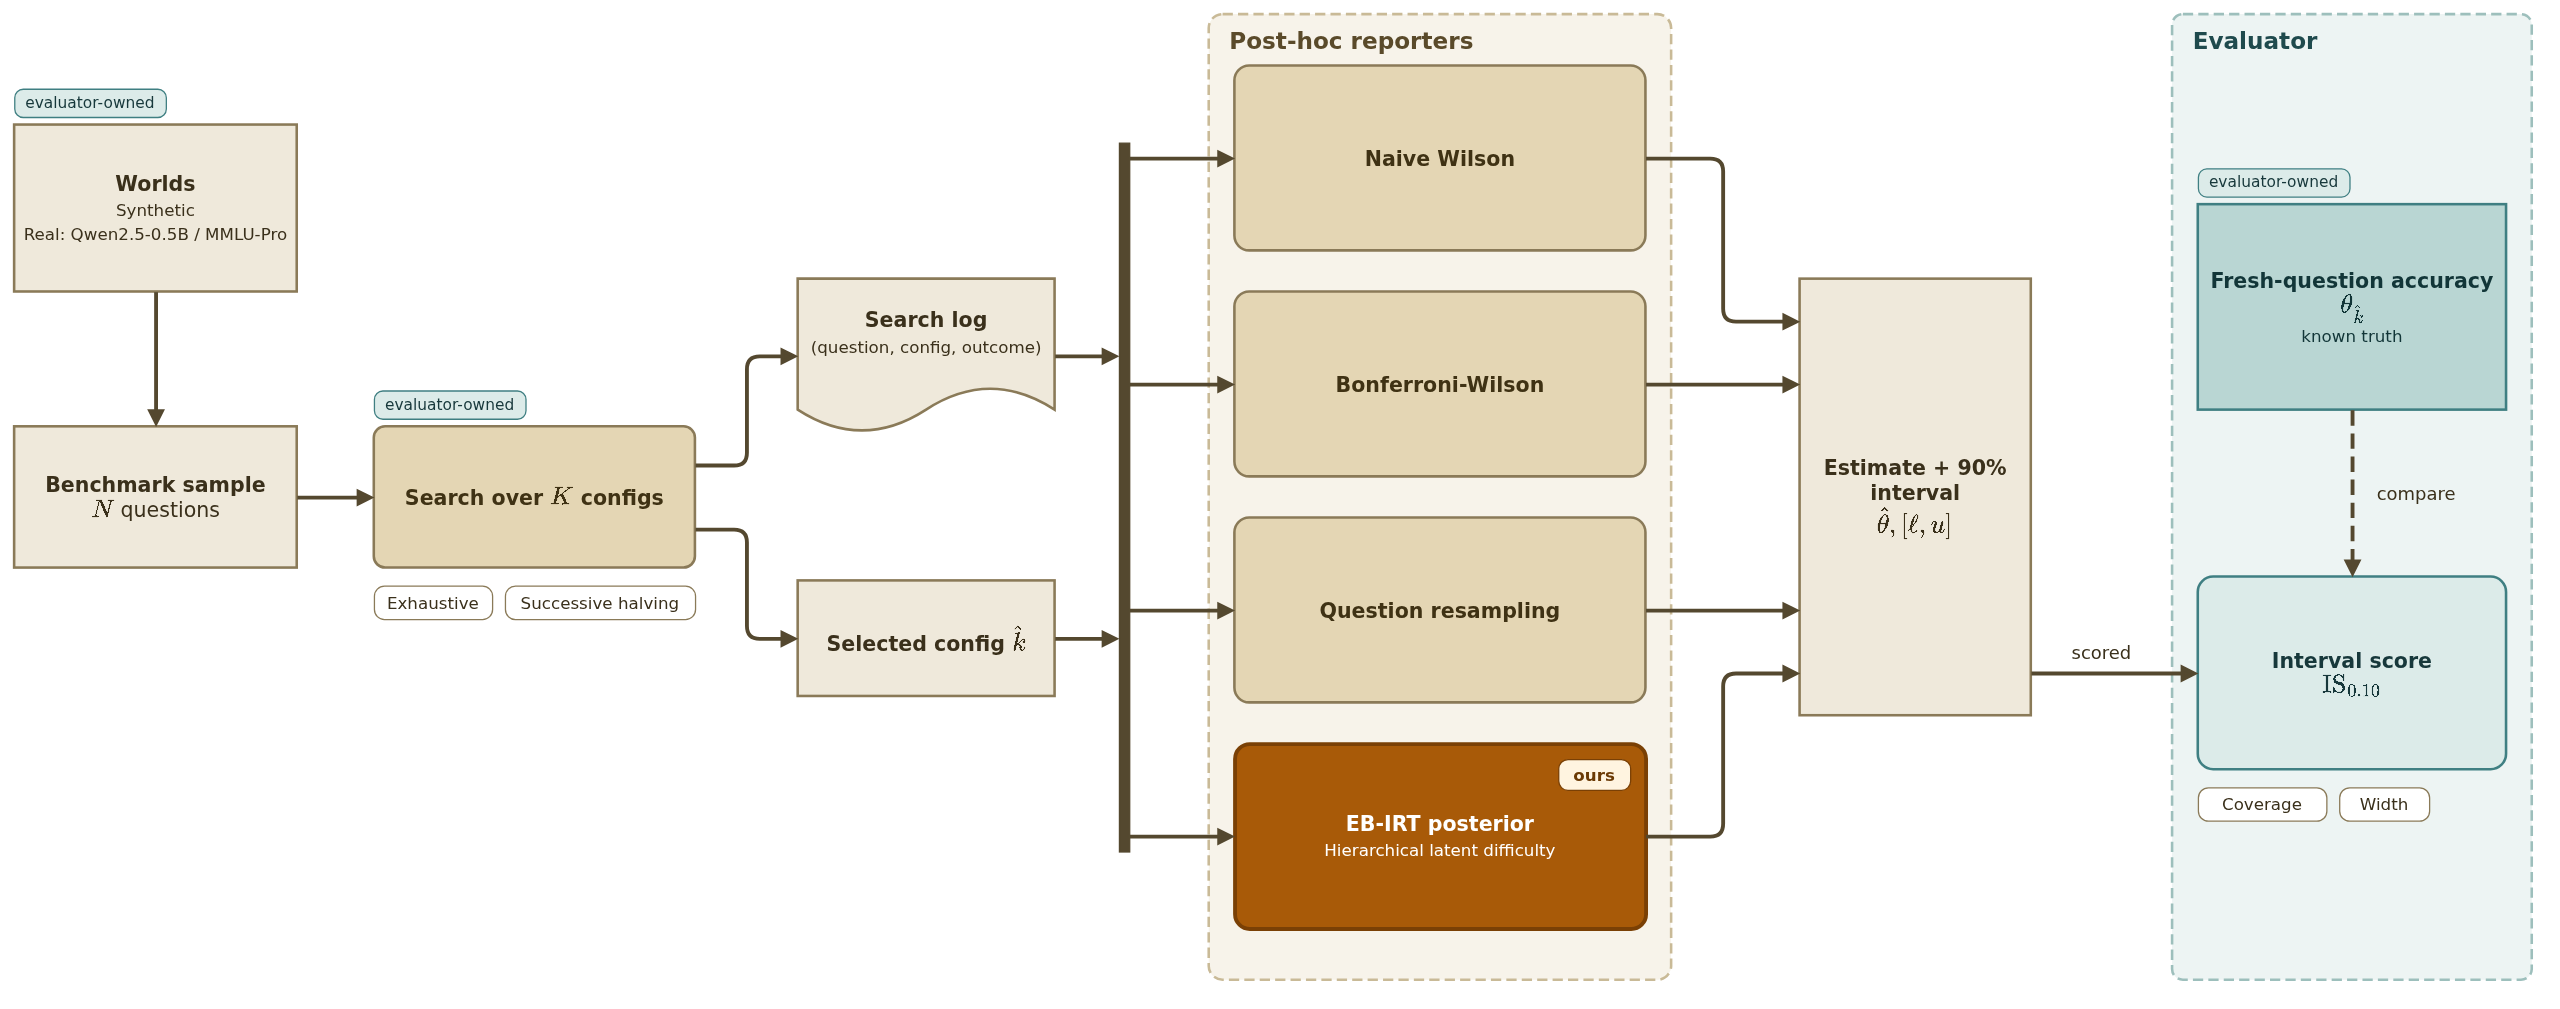
\includegraphics[width=\textwidth]{figures/overview_schematic.png}
\caption{Reporting after search. A benchmark sample of $N$ questions is used to search $K$ configurations; the search log and the selected configuration are passed to a reporter, which returns a point estimate and a 90\% interval for the selected configuration's accuracy on fresh questions. We compare the naive Wilson interval, a Bonferroni-widened interval, a question-resampling optimism correction, and the EB-IRT posterior interval, all scored against known truth.}
\label{fig:overview}
\end{figure}

\section{Related Work}
\textbf{Adaptive data analysis.} Reusing a holdout set across adaptively chosen analyses invalidates standard inference. \citet{Dwork2014PreservingSV,Dwork2015GeneralizationIA} showed that differential-privacy-style noise preserves validity, \citet{Dwork2015TheRH} gave the reusable holdout, \citet{Feldman2017CalibratingNT} calibrated the noise to variance, and \citet{Hardt2014Hard} showed that preventing false discovery in fully interactive analysis is computationally hard. The Ladder \citep{Blum2015Ladder} reports leaderboard scores of repeated submissions through a thresholded mechanism. These methods change \emph{what is released} to the analyst. Our reporter instead leaves the search untouched and corrects the report afterwards from the log; it does not provide their worst-case guarantees, and we do not study adaptive reporting across several released scores.

\textbf{Inference after selection.} Post-selection inference constructs valid intervals for selected targets \citep{Berk2013ValidPSI}; \citet{Andrews2024InferenceOnWinners} study inference on the best-performing unit, the direct statistical analogue of a best-of-search score; and \citet{Chernozhukov2013Gaussian} give Gaussian approximations for maxima that underlie bootstrap critical values. Empirical-Bayes shrinkage \citep{Efron1973Stein} and its connection to selection bias \citep{Efron2011Tweedie} motivate our use of a hierarchical model. The bootstrap optimism correction \citep{Efron1997Bootstrap632} motivates the question-resampling baseline. In machine learning, the optimism of a score used to choose among candidates is a documented source of selection bias in model selection \citep{Cawley2010Overfitting}, and benchmark overfitting under repeated reuse has been probed empirically, on image classification by collecting a fresh test set \citep{Recht2019ImageNet} and by studying how the number of classes affects overfitting from test-set reuse \citep{Feldman2019MultipleClasses}. We study the same optimism for searched LLM configurations, with ground truth supplied by the evaluator.

\textbf{Prompt search and LLM evaluation.} DSPy \citep{Khattab2023DSPy} and MIPRO \citep{OpsahlOng2024MIPRO} automate prompt and pipeline optimization, LLM-driven optimizers generate and select instructions by their score on task examples \citep{Zhou2022APE,Yang2023OPRO}, best-arm formulations bound evaluation cost \citep{Shi2024PromptBAI}, successive halving \citep{Jamieson2016SuccessiveHalving} is a standard budget allocator, performance is sensitive to prompt formatting \citep{Sclar2023Quantifying}, multi-prompt evaluation can be made sample-efficient \citep{Polo2024EfficientMultiPrompt}, item response theory has been used to analyse machine-learning classifiers at the instance level \citep{MartinezPlumed2019IRTinAI}, and error bars on benchmark scores have been advocated \citep{Miller2024ErrorBars}. None of these works supplies a post-search score with selection-aware uncertainty. We use the Wilson interval \citep{Wilson1927Probable} for the baselines.

\section{Method}\label{sec:method}
\subsection{Problem setup and success criterion}
A system is searched over $K$ configurations on $N$ benchmark questions. A searcher produces a log $\mathcal L=\{(q_i,k_i,y_i)\}$ of question indices, configuration indices and binary outcomes, and selects $\hat k$ as a function of $\mathcal L$ only. The target is the selected configuration's accuracy $\theta_{\hat k}$ on fresh questions, which the evaluator knows. A reporter receives $\mathcal L$, $\hat k$, $N$, $K$, the searcher tag and an anonymous subject code per question, and returns $(\hat\theta,\ell,u)$ with $0\le \ell\le\hat\theta\le u\le 1$. We score the interval with the interval score at level $1-\alpha=0.90$,
\begin{equation}
\IS_\alpha(\ell,u;\theta)=(u-\ell)+\tfrac{2}{\alpha}\,(\ell-\theta)_+ + \tfrac{2}{\alpha}\,(\theta-u)_+ ,
\end{equation}
which is a proper scoring rule minimized in expectation by the $\alpha/2$ and $1-\alpha/2$ predictive quantiles \citep{Gneiting2007Scoring}. A missed replication costs $20$ per unit of miss distance, so over-narrow intervals are penalized heavily. We also report coverage, mean width, signed bias of $\hat\theta$ and RMSE. A reporter that fails on a replication receives the worst-case score $20$.

\subsection{Design rationale}
The naive reporter returns the selected configuration's observed accuracy $\hat p_{\hat k}$ with a Wilson interval. Two effects make it unreliable. First, $\hat p_{\hat k}$ is the maximum of noisy estimates, so $\mathbb E[\hat p_{\hat k}-\theta_{\hat k}]>0$ (winner's curse); the effect grows when true differences between configurations are small relative to sampling noise, as in a null world. Second, the Wilson interval treats $\hat p_{\hat k}$ as a fixed-configuration estimate and ignores selection, so it is too short for its nominal level. We expect an estimator that pools information across configurations and questions to shrink the winner's estimate toward the bulk, and a posterior over $\theta_{\hat k}$ to give an interval whose length reflects how little the log says about the selected configuration.

\subsection{EB-IRT reporter}
% @evidence[[analysis/kappa_values.json]]
% @evidence[[source_evidence/reporter_eb_irt/reporter.py]]
\textbf{Model.} With $\sigma$ the logistic function, each logged outcome follows
\begin{equation}
y_{qk}\sim\mathrm{Bernoulli}\big(\sigma(a_k-b_q)\big),\quad a_k\sim\mathcal N(0,\tau^2),\quad b_q\sim\mathcal N(m_{s(q)},s^2),
\end{equation}
This is a Rasch-type item response model with hierarchical priors, whose item parameters are classically estimated by marginal maximum likelihood with EM \citep{Bock1981MML}; our fit below instead alternates Newton sweeps over configuration and question parameters with Laplace-corrected variance updates. Here $a_k$ is a configuration effect, $b_q$ a question difficulty and $m_{s}$ the mean difficulty of subject $s$ (the question's subject code; synthetic worlds have a single code). Subject means are shrunk toward the global mean with five pseudo-questions. The fresh-question accuracy of configuration $k$ is $\theta_k=\mathbb E_b[\sigma(a_k-b)]$, where $b$ is drawn from the mixture of subjects weighted by the observed subject frequencies.

\textbf{Empirical-Bayes fit.} Using only the sparse triples, we alternate damped Newton sweeps for $(a,b)$ with variance updates $\tau^2\leftarrow\frac1K\big(\sum_k\hat a_k^2+\sum_k S_k^{-1}\big)$ and $s^2\leftarrow\frac1N\big(\sum_q(\hat b_q-m_{s(q)})^2+\sum_q H_q^{-1}\big)$, where $S_k$ is the Schur-complement posterior precision of $a_k$ after integrating out difficulties and $H_q$ the diagonal Hessian for $b_q$. These Laplace corrections stop $\tau^2$ from collapsing or inflating. Fitting uses bincount-based vector operations, so exhaustive and halving logs share one code path; the fit stops after at most 30 sweeps or a 1.5\,s wall-clock budget.

\textbf{Ignorability.} Exhaustive search and successive halving choose which entries to observe and which configuration to select using only previously observed outcomes. The likelihood of the log is therefore unaffected by the design, and a likelihood-based posterior is valid under either searcher without a searcher-specific correction, provided the model is adequately specified. This is a motivation, not a proof for the real-outcome worlds, whose subject-by-configuration structure a one-dimensional difficulty model only approximates.

\textbf{Posterior interval.} We draw 400 samples of $(a_{\hat k},\text{level shift},\log s)$ from Laplace approximations, integrate over fresh difficulties with 21 Gauss--Hermite nodes and each subject, and obtain draws of $\theta_{\hat k}$. The estimate is their mean $\hat\theta$; with $q_{0.05},q_{0.95}$ the posterior quantiles, the reported interval is
\begin{equation}
\ell=\hat\theta-\kappa\,(\hat\theta-q_{0.05})_+,\qquad u=\hat\theta+\kappa\,(q_{0.95}-\hat\theta)_+ ,
\end{equation}
with a width factor $\kappa(N,K)=\kappa_0\,\big(1+0.25\min(1,\sqrt{50/N})\big)\big(1+0.03\log_2(K/2)\big)$, where $\kappa_0=1.20$ when the log carries subject codes (real outcomes) and $1.12$ otherwise. The constants are fixed in the source; they are design priors that widen the interval to compensate for ignored hyperparameter uncertainty and misspecification, not values fitted to the final worlds. Over the cases studied $\kappa$ ranges from 1.43 to 1.63 (Table~\ref{tab:kappa} in the Supplement), so intervals are roughly 40--60\% wider than raw posterior quantiles. Because $\kappa$ acts only around $\hat\theta$, bias comparisons with the naive estimate reflect the posterior mean alone, whereas interval width and coverage reflect the posterior and $\kappa$ jointly; we did not evaluate $\kappa=1$.

\textbf{Degenerate worlds.} If every outcome is zero the reporter returns estimate $0$ and upper bound $\min(3/n_{\hat k},0.02)$; if $\hat k$ was never observed it returns the pooled mean $\pm0.25$; any exception falls back to a widened Wilson interval.

\subsection{Compared reporters}\label{sec:baselines}
All baselines are computed by the evaluator from the same log. \emph{Naive Wilson}: observed accuracy of $\hat k$ with a 90\% Wilson interval. \emph{Bonferroni-Wilson}: the same estimate with the Wilson critical value taken at level $1-\alpha/(2K)$. \emph{Resampling}: 100 random half-splits; on each, the best configuration on one half is re-scored on the other, the mean score gap $g$ is rescaled to $\hat p_{\hat k}-g/\sqrt2$, and a Wilson interval is placed around it.

\subsection{Experimental protocol}\label{sec:protocol}
% @evidence[[source_evidence/evaluator/evaluate_final.py#CASES]]
% @evidence[[source_evidence/evaluator/final_manifest.json]]
% @evidence[[analysis/reconstructed_baselines.json#max_abs_diff_vs_recorded]]
% @evidence[[paper_data.json#final.metric.completed_replication_fraction]]
\textbf{Worlds.} \emph{Synthetic} worlds draw a base accuracy uniformly from $[0.25,0.75]$ and per-configuration accuracies with spread $0.03$; outcomes follow a Gaussian copula with latent correlation $0.5$ across configurations, and the truth is the selected configuration's accuracy. \emph{Real} worlds use a cached $1500\times24$ binary tensor of Qwen2.5-0.5B-Instruct answers on MMLU-Pro (24 prompt configurations: four instruction wordings $\times$ three demonstration settings $\times$ two answer-prefix formats; revisions in the Supplement). Each replication samples $N$ questions without replacement, permutes configuration labels, searches, and takes as truth the selected configuration's accuracy on the remaining pool questions. \emph{Controls}: N1 is a synthetic world with identical configurations; N2 is the real pool with each question's configuration columns reassigned by a random derangement to break configuration effects; Z1 is an all-zero world with $K=8$. In any null world no configuration is better, so a reporter should neither invent signal nor lose coverage.

\textbf{Cases and searchers.} Table~\ref{tab:cases} lists the cases. \emph{Exhaustive} search evaluates every configuration on every question and selects the highest total; \emph{successive halving} works with a nominal budget of $N\!\cdot\!K$ evaluations over $\lceil\log_2K\rceil$ rounds, discarding the lower half of the survivors each round, so configurations eliminated early are observed on few questions and the log is sparse. Each case has $R=30$ replications ($R=10$ for Z1).

\textbf{Aggregation and uncertainty.} Per-case values average replications; the primary aggregate averages P1--P2 (synthetic, weight 0.4) and P3--P6 (real, weight 0.6) within family. The sealed evaluation uses eight seeds (9101--9108), each running all nine cases. We report mean $\pm$ standard deviation of seed-level values and, for reporter differences, paired seed-level differences. The evaluator records interval score, bias, coverage and width for the EB-IRT reporter, but only the interval scores of the three baselines and the bias of the naive reporter. All other baseline quantities (baseline coverage and width, and the bias of the Bonferroni and resampling reporters) are replay-derived: we replayed the evaluator's own deterministic world, search and baseline code, which reproduced the recorded baseline interval scores and the recorded naive bias exactly (maximum absolute difference 0). The replay-derived values are not checked against any evaluator record. Per-case records carry an unverified diagnostics label from the evaluator, so we treat aggregate metrics as authoritative and per-case values as supporting. The reporter was frozen before the sealed evaluation, and the evaluation completed all replications (completed fraction 1.0).

\section{Results}\label{sec:results}
\subsection{Optimism of best-of-search reporting}\label{sec:gap}
% @evidence[[analysis/final_per_case.json#aggregate_primary.naive_bias]]
% @evidence[[analysis/final_per_case.json#cases]]
% @evidence[[analysis/final_per_case.json#naive_bias_searcher_diff]]
% @evidence[[analysis/reconstructed_baselines.json#aggregate_primary]]
% @evidence[[source_evidence/evaluator/final_manifest.json#per_config_pool_accuracy]]
Averaged over P1--P6 the naive estimate exceeds the fresh-question accuracy by $0.0366\pm0.0029$ (Table~\ref{tab:aggregate}). Its nominal 90\% Wilson interval contains the truth in $0.713\pm0.048$ of replications, and in no primary case does it reach 0.82 (Table~\ref{tab:cases}). The Bonferroni-widened interval fixes coverage ($0.962$) but spends width: $0.190$ against $0.129$ for EB-IRT.

\emph{Question budget.} On the three real exhaustive cases ($K=24$) the naive bias falls monotonically with $N$: $0.051$ at $N=60$ (P5), $0.022$ at $N=200$ (P3), $0.009$ at $N=600$ (P6) (Figure~\ref{fig:biascov}a). The optimism at $N=60$ is of the same order as the spread of the 24 configurations' pool accuracies ($0.107$ to $0.166$ in the final pool); we did not measure how the optimism relates to true between-configuration differences.

\emph{World.} Optimism is larger when configurations do not truly differ: in the synthetic null N1 the naive bias is $0.067$ against $0.049$ in P1 (same $N$, $K$, searcher), and in the permuted real null N2 it is $0.034$ against $0.022$ in P3. This is the winner's-curse pattern expected when selection is among near-equals; we did not test it causally.

\emph{Searcher and $K$.} Under halving the naive bias is $0.054$ (P2) and $0.025$ (P4), versus $0.049$ (P1) and $0.022$ (P3) under exhaustive search in matched worlds. The matched paired differences ($+0.004\pm0.012$ and $+0.003\pm0.008$ across seeds) are small relative to seed spread; aggregated over searcher-specific cases the naive bias is $0.036$ under both. We cannot separate the effect of $K$ because it is confounded with the world (32 synthetic, 24 real, 8 constant).

\subsection{Main comparison: sealed final evaluation}
% @evidence[[paper_data.json#final.metric.mean_interval_score]]
% @evidence[[paper_data.json#final.metric.rmse]]
% @evidence[[paper_data.json#final.qualification.status]]
% @evidence[[analysis/final_per_case.json#paired_diff_aggregate]]
\begin{table}[t]
\centering
\caption{Sealed final evaluation, primary cases P1--P6 (0.4 synthetic / 0.6 real), mean $\pm$ standard deviation over eight seeds. The interval score is at level 0.90 (lower is better); coverage should be near 0.90. Bonferroni-Wilson shares the naive point estimate. Baseline coverage, width and the resampling bias are replay-derived from the evaluator's code, not evaluator-recorded (Section~\ref{sec:protocol}).}
\label{tab:aggregate}
\small
% @evidence[[tables/aggregate.tex]]
% @evidence[[paper_data.json#final.metric.mean_interval_score]]
% @evidence[[paper_data.json#final.metric.naive_baseline_score]]
% @evidence[[paper_data.json#final.metric.bonferroni_baseline_score]]
% @evidence[[paper_data.json#final.metric.resample_baseline_score]]
% @evidence[[paper_data.json#final.metric.coverage]]
% @evidence[[paper_data.json#final.metric.naive_signed_bias]]
% @evidence[[analysis/final_per_case.json]]
% @evidence[[analysis/reconstructed_baselines.json]]
\begin{tabular}{lcccc}
\toprule
Reporter & Interval score $\downarrow$ & Coverage & Mean width & Signed bias \\
\midrule
Naive Wilson & 0.2202$\pm$0.0234 & 0.713$\pm$0.048 & 0.109 & 0.0366$\pm$0.0029 \\
Bonferroni-Wilson & 0.1974$\pm$0.0036 & 0.962$\pm$0.012 & 0.190 & 0.0366$\pm$0.0029 \\
Resampling & 0.2461$\pm$0.0251 & 0.748$\pm$0.020 & 0.104 & $-$0.0209$\pm$0.0030 \\
\textbf{EB-IRT (ours)} & 0.1449$\pm$0.0040 & 0.929$\pm$0.008 & 0.129 & 0.0121$\pm$0.0027 \\
\bottomrule
\end{tabular}
\end{table}

EB-IRT attains a mean interval score of $0.1449$ against $0.2202$ (naive), $0.1974$ (Bonferroni-Wilson) and $0.2461$ (resampling) (Table~\ref{tab:aggregate}), with coverage $0.929$ and RMSE $0.0348$. Its score is lower than each baseline's in all eight seeds; paired seed-level differences are $0.075\pm0.021$ (naive), $0.053\pm0.004$ (Bonferroni) and $0.101\pm0.023$ (resampling). Its aggregate bias, $0.0121\pm0.0027$, removes about two thirds of the naive optimism. The evaluator's qualification outcome for this run is ``qualified'' with status ``completed''. Gate diagnostics beyond that outcome are not available to us, and the outcome does not by itself establish validity beyond the studied worlds.

\begin{figure}[t]
\centering
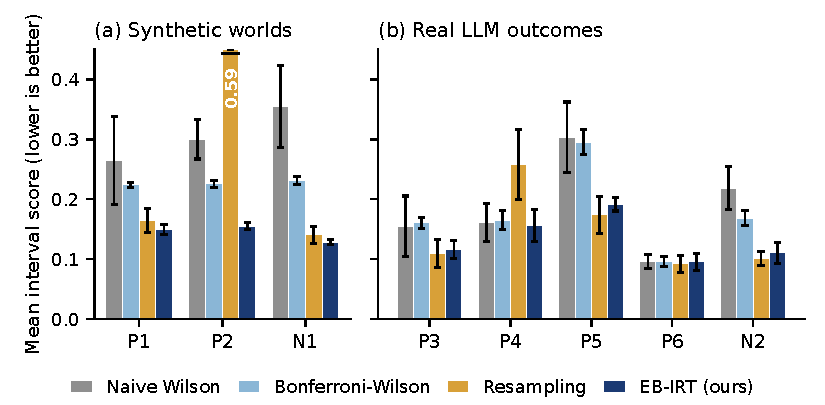
\includegraphics[width=\textwidth]{figures/per_case_interval_score.pdf}
\caption{Mean interval score per case (lower is better) for four reporters; bars show mean over eight seeds, whiskers one standard deviation across seeds. (a) Synthetic worlds including the null N1. (b) Real outcomes including the permuted null N2. The resampling bar for P2 is clipped (value 0.59).}
\label{fig:perCase}
\end{figure}

\begin{table}[t]
\centering
\caption{Per-case interval score (mean over eight seeds; best per row in bold) and coverage of the naive and EB-IRT intervals. ``exh.'' exhaustive search, ``halv.'' successive halving. Seed standard deviations are in the Supplement.}
\label{tab:cases}
\small
\setlength{\tabcolsep}{4pt}
% @evidence[[tables/per_case.tex]]
% @evidence[[analysis/final_per_case.json]]
% @evidence[[analysis/reconstructed_baselines.json]]
\begin{tabular}{llrrcccccc}
\toprule
Case & World, search & $N$ & $K$ & Naive & Bonf. & Resamp. & EB-IRT & Cov.\ naive & Cov.\ EB-IRT \\
\midrule
P1 & synthetic, exh. & 150 & 32 & 0.264 & 0.224 & 0.164 & \textbf{0.150} & 0.65 & 0.96 \\
P2 & synthetic, halv. & 150 & 32 & 0.300 & 0.225 & 0.592 & \textbf{0.155} & 0.61 & 0.96 \\
P3 & real, exh. & 200 & 24 & 0.155 & 0.161 & \textbf{0.109} & 0.116 & 0.81 & 0.94 \\
P4 & real, halv. & 200 & 24 & 0.161 & 0.165 & 0.258 & \textbf{0.156} & 0.77 & 0.89 \\
P5 & real, exh. & 60 & 24 & 0.303 & 0.295 & \textbf{0.174} & 0.192 & 0.71 & 0.98 \\
P6 & real, exh. & 600 & 24 & 0.096 & 0.096 & \textbf{0.092} & 0.096 & 0.78 & 0.83 \\
\midrule
N1 & synth.\ null, exh. & 150 & 32 & 0.354 & 0.231 & 0.140 & \textbf{0.128} & 0.47 & 0.97 \\
N2 & real null, exh. & 200 & 24 & 0.218 & 0.168 & \textbf{0.102} & 0.111 & 0.62 & 0.89 \\
Z1 & all-zero, exh. & 100 & 8 & 0.026 & 0.059 & 0.026 & \textbf{0.020} & 1.00 & 1.00 \\
\bottomrule
\end{tabular}
\end{table}

\subsection{Where the gain is large, and where it is not}
% @evidence[[analysis/final_per_case.json#by_searcher]]
% @evidence[[analysis/final_per_case.json#cases]]
% @evidence[[analysis/reconstructed_baselines.json#cases]]
Figure~\ref{fig:perCase} and Table~\ref{tab:cases} show a heterogeneous picture, which the aggregate hides.

\emph{Large gains.} On synthetic worlds and at small $N$ EB-IRT lowers the naive interval score by 37--48\% (P1: $0.150$ vs $0.264$; P2: $0.155$ vs $0.300$; P5: $0.192$ vs $0.303$) with coverage at or above nominal. It also beats Bonferroni-Wilson by $0.07$--$0.10$ in P1, P2 and P5 in every seed.

\emph{No gain over naive.} In real-outcome halving (P4) the three Wilson-style scores are close ($0.156$ vs naive $0.161$, Bonferroni $0.165$); the paired advantage over naive is $0.005$ and EB-IRT wins in six of eight seeds. Its point estimate is \emph{more} biased than the naive one there ($0.031$ vs $0.025$) and its coverage is $0.89$, slightly below nominal but within seed noise (seed s.d.\ $0.03$ over eight seeds). At $N=600$ (P6) all Wilson-style reporters score $0.096$ and the naive bias is already small ($0.009$ vs $0.011$ for EB-IRT).

\emph{Resampling is as good under exhaustive search.} Restricting the aggregate to exhaustive-search cases (P1 and P3, P5, P6, same weights) gives interval scores of $0.1406$ for EB-IRT and $0.1405$ for resampling, against $0.2166$ for naive: a tie. In the real exhaustive cases P3, P5 and N2 resampling is slightly better ($0.109$, $0.174$, $0.102$ vs $0.116$, $0.192$, $0.111$), and EB-IRT is the better of the two in only 2, 1 and 1 of eight seeds respectively. The aggregate advantage over resampling therefore comes from halving: on halving cases resampling scores $0.3916$ against $0.1556$, because it over-corrects the sparse log (replay-derived bias $-0.067$ in P2 and $-0.031$ in P4; replay-derived coverage $0.44$ and $0.61$). EB-IRT is the more robust reporter across searchers, not uniformly the more accurate.

\begin{figure}[t]
\centering
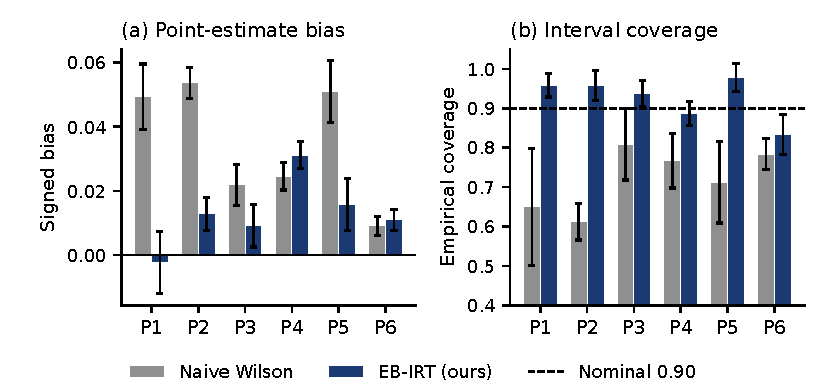
\includegraphics[width=\textwidth]{figures/bias_and_coverage.pdf}
\caption{Diagnostics for the primary cases (mean over eight seeds, whiskers one standard deviation across seeds). (a) Signed bias of the point estimate for the naive and EB-IRT reporters. (b) Empirical coverage of the 90\% intervals; dashed line marks the nominal level. Naive coverage is replayed from the evaluator's code.}
\label{fig:biascov}
\end{figure}

\begin{figure}[t]
\centering
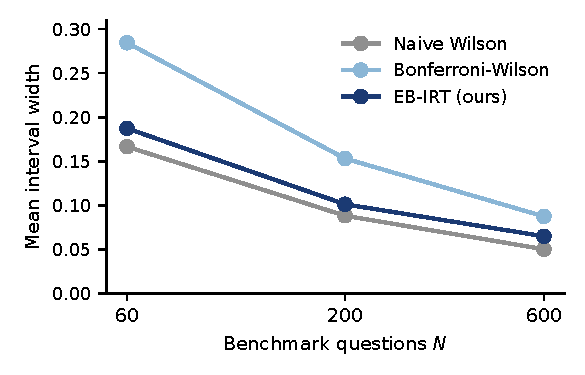
\includegraphics[width=0.7\textwidth]{figures/width_vs_n.pdf}
\caption{Mean interval width on the real exhaustive cases ($K=24$) as the number of benchmark questions grows (mean over eight seeds). EB-IRT is wider than the naive interval by a factor of 1.1--1.3 at each $N$ and much narrower than Bonferroni-Wilson. Naive and Bonferroni widths are replayed from the evaluator's code.}
\label{fig:width}
\end{figure}

\emph{Residual bias and miscalibrated width.} EB-IRT's signed bias is positive in five of six primary cases (range $0.009$--$0.031$) and slightly negative only in P1 ($-0.002\pm0.010$) (Figure~\ref{fig:biascov}a); shrinkage removes most, not all, of the winner's curse. Coverage varies from $0.98$ (P5) and $0.96$ (P1, P2) down to $0.89$ (P4) and $0.83$ (P6) (Figure~\ref{fig:biascov}b). Interval width shrinks with $N$ for all reporters (Figure~\ref{fig:width}): EB-IRT is $0.187$, $0.101$ and $0.065$ wide at $N=60$, $200$, $600$, against $0.167$, $0.088$ and $0.050$ for the naive interval and $0.284$, $0.153$ and $0.088$ for Bonferroni-Wilson. The aggregate coverage of $0.929$ is thus an average of over- and under-coverage rather than evidence of calibration in each regime: the fixed width factor over-widens the synthetic and small-$N$ cases and under-widens the largest-$N$ real case. At $N=600$ the target itself is measured on the remaining 900 pool questions, a finite-sample noise that no reporter here models and that matters most where intervals are narrowest; we did not test how much of the P6 shortfall it explains.

\subsection{Negative controls}\label{sec:controls}
% @evidence[[analysis/final_per_case.json#cases.N1]]
% @evidence[[analysis/final_per_case.json#cases.N2]]
% @evidence[[analysis/final_per_case.json#cases.Z1]]
% @evidence[[paper_data.json#final.metric.null_control_abs_bias]]
% @evidence[[paper_data.json#final.metric.constant_control_error]]
In the synthetic null N1 EB-IRT has coverage $0.971$ and interval score $0.128$ against $0.354$ for naive, whose coverage is $0.47$. In the permuted real null N2 EB-IRT has coverage $0.887$ and interval score $0.111$ (naive $0.218$, resampling $0.102$). In both nulls its bias is $0.017$: shrinkage does not reduce the estimate fully to the common mean, and the controls average $0.0173$ in absolute bias. In the constant-zero world Z1 the reporter returns exactly zero with interval $[0,0.02]$ (absolute estimate error $0$, interval score $0.020$ against $0.026$ naive and $0.059$ Bonferroni). The reporter therefore does not manufacture signal in null worlds, but its null coverage in the real world sits at the same $0.89$ as in P4.

\subsection{Reporter variants considered during development}
% @evidence[[analysis/search_variants.json]]
Two alternative designs were evaluated in the development setting (four seeds, cases P1--P4 with controls) alongside EB-IRT: a parametric-bootstrap pivot calibration of the interval, and an extension with configuration-by-subject random effects. Table~\ref{tab:variants} shows that narrower intervals do not pay: the bootstrap variant has the smallest width ($0.085$) but coverage $0.77$ and a higher interval score ($0.1562$) than EB-IRT ($0.1480$), and the interaction effects did not improve it ($0.1519$, coverage $0.893$). Each was evaluated once, so these differences are not a significance ranking; these runs are kept separate from the sealed evaluation, in which only EB-IRT was evaluated.

\begin{table}[t]
\centering
\caption{Development-setting comparison of reporter variants (four seeds; P1--P4 primary, N1--N2 for null-control coverage); single evaluation each, not a significance ranking. Baseline rows are the evaluator's reporters in the same setting.}
\label{tab:variants}
\small
% @evidence[[tables/search_variants.tex]]
% @evidence[[analysis/search_variants.json]]
\begin{tabular}{lccccc}
\toprule
Variant & Interval score & Coverage & Width & Bias & Null-control cov. \\
\midrule
EB-IRT (frozen selection) & 0.1480 & 0.915 & 0.124 & 0.0143 & 0.933 \\
+ config$\times$subject effects & 0.1519 & 0.893 & 0.120 & 0.0152 & 0.908 \\
Bootstrap pivot calibration & 0.1562 & 0.770 & 0.085 & 0.0092 & 0.738 \\
\midrule
Naive Wilson & 0.2321 & -- & -- & 0.0366 & -- \\
Bonferroni-Wilson & 0.1961 & -- & -- & -- & -- \\
Resampling & 0.2732 & -- & -- & -- & -- \\
\bottomrule
\end{tabular}
\end{table}

\section{Discussion and Limitations}\label{sec:limits}
% @evidence[[analysis/final_per_case.json#aggregate_primary]]
% @evidence[[analysis/final_per_case.json#paired_diff_aggregate]]
% @evidence[[analysis/reconstructed_baselines.json#aggregate_primary]]
\textbf{What the evidence supports.} In the studied worlds, best-of-search reporting is optimistic by $0.037$ absolute on average and its nominal interval is badly calibrated, a gap that depends on the question budget and on how distinguishable the configurations are. A hierarchical posterior interval fitted to the log lowers the interval score by about a third relative to the naive report and by a quarter relative to Bonferroni-Wilson with lower width. These statements hold for eight seeds of a sealed run that completed with a qualified outcome.

\textbf{How to test a reporter (Q2).} Our results suggest what a reliability test should contain. (a) Worlds with known truth, so that coverage and bias are measured rather than inferred. (b) Interval score together with coverage, since either alone is gamed by extreme widths: Bonferroni-Wilson reaches coverage $0.96$ only by being $47\%$ wider than EB-IRT. (c) Results by regime (search procedure, question budget, world), because the aggregate coverage of $0.929$ conceals cases from $0.83$ to $0.98$. (d) Negative controls: a null world to catch invented signal, a constant world to catch degenerate behaviour. (e) Seed-level uncertainty and paired differences between reporters, since the naive and resampling scores vary across seeds with standard deviations of $0.023$ and $0.025$, against $0.004$ for EB-IRT. (f) Baselines matched to the searcher: against resampling alone, the exhaustive-search verdict (a tie) differs from the halving verdict (a large gain).

\textbf{What it does not support.} (1) \emph{Generality}: one 0.5B model whose accuracies (0.11--0.17) are close to the 10-option chance level of 0.10, one benchmark, one prompt family; the configuration spread and the optimism may differ for stronger models. (2) \emph{Searchers}: only evaluator-owned exhaustive and halving searchers; no DSPy or MIPRO run, and no adaptive reporting of several scores in the manner of the Ladder. (3) \emph{Decisions}: we measured the gap in a single configuration's accuracy, not whether it reverses rankings or deployment decisions; coverage and miss penalties show that reported numbers are unreliable, not how often a conclusion changes. (4) \emph{Attribution}: the $\kappa$ widening is hand-set and was never switched off, and subject means, EB variances and the Laplace correction were not ablated, so we cannot say how much coverage comes from the model versus the widening. The bias comparison is unaffected by $\kappa$. (5) \emph{Misspecification}: one-dimensional difficulty is a poor fit for real subject-by-configuration structure; the extension that added such structure did not help in development. (6) \emph{Residual failures}: undercoverage at $N=600$ ($0.83$, seed s.d.\ $0.05$), slightly sub-nominal coverage in real-outcome halving ($0.89$, within seed noise), positive bias in null worlds, and no gain over naive in P4 and P6. (7) \emph{Theory}: ignorability is an argument, not a guarantee for misspecified models, and we offer no coverage theorem. (8) \emph{Provenance}: the real outcome tensors were produced by the task authors and not regenerated, per-case diagnostics are labelled unverified, and the evaluator's gate diagnostics beyond the outcome are unavailable, so we make no claim about why individual checks passed. The qualified outcome does not turn these limits into guarantees.

\section{Conclusion}
% @evidence[[paper_data.json#final.metric.mean_interval_score]]
% @evidence[[paper_data.json#final.metric.naive_signed_bias]]
% @evidence[[analysis/reconstructed_baselines.json#aggregate_primary.naive_cov]]
After automatic prompt search, a score reported on the search sample is an optimistic and over-confident description of fresh-question accuracy: across the studied worlds the naive best-of-search estimate is too high by about 0.04 on average, and its nominal 90\% interval contains the truth about 71\% of the time. A searcher-agnostic empirical-Bayes latent-difficulty posterior interval, computed from the search log alone, cut the interval score from 0.220 to 0.145 in a sealed eight-seed evaluation whose qualification outcome is ``qualified'', and reduced the bias by about two thirds. The improvement concentrates in synthetic worlds, at small question budgets, and under halving relative to resampling; for real exhaustive search a question-resampling correction is equally good, and for real halving and large question budgets the new reporter is no better than the naive interval, with coverage clearly below nominal only at 600 questions (0.83) and slightly below it under real halving (0.89). We therefore recommend the reporter as a conditional, searcher-agnostic default for small samples, together with the evaluation protocol: known truth, null and constant controls, coverage next to interval score, and seed-level uncertainty. Open questions are whether the optimism alters rankings, how much of the coverage is owed to the width calibration, and whether the pattern holds for stronger models and real prompt optimizers.

% IMPORTANT: \clearpage flushes all pending floats before references so that
% body-page counting excludes reference-only pages.  Do NOT remove.
\clearpage
\bibliography{references}
\bibliographystyle{paper}

\clearpage
\appendix
\section{Supplementary Information}
\subsection{Estimator details and hyperparameters}
The reporter is a single Python module with NumPy only. Fixed constants: at most 30 EB sweeps (three damped Newton steps for $a$ and for $b$ per sweep, steps clipped to $\pm1$) with a 1.5\,s wall-clock guard; $\tau^2\in[10^{-4},4]$, $s^2\in[10^{-2},25]$; initial $\tau^2=0.25$, $s^2=1$; five pseudo-questions for subject means; 400 posterior draws; 21 Gauss--Hermite nodes; level-shift draws with standard deviation $s/\sqrt N$ and $\log s$ perturbations with standard deviation $1/\sqrt{2N}$. The prior variance of $a_{\hat k}$ is floored at $0.3$ times the median inverse Schur precision so that near-equal configurations still receive an interval reflecting sampling noise. The world is treated as ``real'' when any subject code is nonzero. Table~\ref{tab:kappa} gives the resulting $\kappa$. The reporter's draws are seeded from the evaluator's reset call. Source: the reporter's module, function \texttt{\_kappa} and \texttt{\_fit\_irt}.
% @evidence[[source_evidence/reporter_eb_irt/reporter.py]]

\begin{table}[h]
\centering
\caption{Width factor $\kappa$ applied around the estimate in each evaluation case (computed from the reporter's own function). It is not used in Z1, where the all-zero rule applies.}
\label{tab:kappa}
\small
% @evidence[[analysis/kappa_values.json]]
\begin{tabular}{lcccc}
\toprule
Case & $N$ & $K$ & Searcher & $\kappa$ \\
\midrule
P1 & 150 & 32 & exhaustive & 1.435 \\
P2 & 150 & 32 & halving & 1.435 \\
P3 & 200 & 24 & exhaustive & 1.495 \\
P4 & 200 & 24 & halving & 1.495 \\
P5 & 60 & 24 & exhaustive & 1.632 \\
P6 & 600 & 24 & exhaustive & 1.425 \\
N1 & 150 & 32 & exhaustive & 1.435 \\
N2 & 200 & 24 & exhaustive & 1.495 \\
\bottomrule
\end{tabular}
\end{table}

\subsection{Evaluation protocol and provenance}
The sealed evaluation runs seeds 9101--9108; each seed runs P1--P6, N1, N2 (30 replications each) and Z1 (10), so $8\times250=2000$ reporter calls. The development setting runs seeds 101--104 with cases P1--P4, N1, N2, Z1. Real worlds: MMLU-Pro revision \texttt{b189ec76\ldots} (MIT licence), Qwen2.5-0.5B-Instruct revision \texttt{7ae55760\ldots} (Apache-2.0), float32 CPU, one deterministic forward pass, prediction by argmax over the ten option-letter logits. Questions are deduplicated by normalized content hash, restricted to 10 options and at most 400 tokens, stratified over 14 subjects; the final pool has 1500 questions and the development pool 599, with no hash overlap between pools or with the demonstration source. The 24 configurations are indexed as (wording $\times$ 3 + demonstration setting) $\times$ 2 + format, with demonstration settings 0-shot and two 3-shot sets from the validation split. Configuration labels are randomly permuted per replication. Aggregate weights are 0.4 synthetic and 0.6 real. The interval score uses $\alpha=0.10$ and a worst case of 20.
% @evidence[[source_evidence/evaluator/final_manifest.json]]
% @evidence[[source_evidence/evaluator/evaluate_final.py#CASES]]

\textbf{Compute.} Evaluator-recorded wall-clock time per seed (250 episodes, covering reporter calls and scoring) averaged $6.2$\,s, about $50$\,s over the eight sealed seeds. No GPU or API was used in this study.
% @evidence[[analysis/final_per_case.json#episode_duration_seconds]]

\subsection{Per-case detail}
Table~\ref{tab:suppcase} gives seed-level spread for all nine cases and Table~\ref{tab:suppbase} the Bonferroni and resampling coverage and width.
\begin{table}[h]
\centering
\caption{Per-case interval score (mean $\pm$ s.d.\ over eight seeds), width and signed bias for EB-IRT and the naive reporter. Naive width is replayed from the evaluator's code.}
\label{tab:suppcase}
\footnotesize
\setlength{\tabcolsep}{4pt}
% @evidence[[analysis/final_per_case.json]]
% @evidence[[analysis/reconstructed_baselines.json]]
\begin{tabular}{lcccccc}
\toprule
Case & IS EB-IRT & IS naive & Width EB-IRT & Width naive & Bias EB-IRT & Bias naive \\
\midrule
P1 & 0.150$\pm$0.009 & 0.264$\pm$0.074 & 0.140 & 0.125 & $-$0.002$\pm$0.010 & 0.049$\pm$0.010 \\
P2 & 0.155$\pm$0.006 & 0.300$\pm$0.033 & 0.150 & 0.125 & 0.013$\pm$0.005 & 0.054$\pm$0.005 \\
P3 & 0.116$\pm$0.015 & 0.155$\pm$0.050 & 0.101 & 0.088 & 0.009$\pm$0.007 & 0.022$\pm$0.006 \\
P4 & 0.156$\pm$0.027 & 0.161$\pm$0.032 & 0.121 & 0.088 & 0.031$\pm$0.004 & 0.025$\pm$0.004 \\
P5 & 0.192$\pm$0.012 & 0.303$\pm$0.059 & 0.187 & 0.167 & 0.016$\pm$0.008 & 0.051$\pm$0.010 \\
P6 & 0.096$\pm$0.014 & 0.096$\pm$0.011 & 0.065 & 0.050 & 0.011$\pm$0.003 & 0.009$\pm$0.003 \\
N1 & 0.128$\pm$0.004 & 0.354$\pm$0.068 & 0.125 & 0.127 & 0.017$\pm$0.004 & 0.067$\pm$0.005 \\
N2 & 0.111$\pm$0.018 & 0.218$\pm$0.035 & 0.089 & 0.087 & 0.017$\pm$0.003 & 0.034$\pm$0.002 \\
Z1 & 0.020$\pm$0.000 & 0.026$\pm$0.000 & 0.020 & 0.026 & 0.000$\pm$0.000 & 0.000$\pm$0.000 \\
\bottomrule
\end{tabular}
\end{table}
\begin{table}[h]
\centering
\caption{Bonferroni-Wilson and resampling reporters per case: interval score (mean $\pm$ s.d.\ over eight seeds), and replayed coverage and width.}
\label{tab:suppbase}
\footnotesize
\setlength{\tabcolsep}{4pt}
% @evidence[[analysis/final_per_case.json]]
% @evidence[[analysis/reconstructed_baselines.json]]
\begin{tabular}{lcccccc}
\toprule
Case & IS Bonf. & IS Resamp. & Cov.\ Bonf. & Cov.\ Resamp. & Width Bonf. & Width Resamp. \\
\midrule
P1 & 0.224$\pm$0.004 & 0.164$\pm$0.020 & 0.98 & 0.90 & 0.221 & 0.127 \\
P2 & 0.225$\pm$0.006 & 0.592$\pm$0.131 & 0.98 & 0.44 & 0.221 & 0.127 \\
P3 & 0.161$\pm$0.009 & 0.109$\pm$0.023 & 0.95 & 0.86 & 0.153 & 0.082 \\
P4 & 0.165$\pm$0.016 & 0.258$\pm$0.058 & 0.95 & 0.61 & 0.153 & 0.075 \\
P5 & 0.295$\pm$0.021 & 0.174$\pm$0.031 & 0.96 & 0.93 & 0.284 & 0.147 \\
P6 & 0.096$\pm$0.008 & 0.092$\pm$0.014 & 0.95 & 0.79 & 0.088 & 0.049 \\
N1 & 0.231$\pm$0.007 & 0.140$\pm$0.014 & 0.97 & 0.95 & 0.224 & 0.127 \\
N2 & 0.168$\pm$0.013 & 0.102$\pm$0.012 & 0.93 & 0.90 & 0.151 & 0.079 \\
Z1 & 0.059$\pm$0.000 & 0.026$\pm$0.000 & 1.00 & 1.00 & 0.059 & 0.026 \\
\bottomrule
\end{tabular}
\end{table}

\subsection{Reproducibility}
All numbers come from the sealed final record and the derived files in \texttt{analysis/}. \texttt{final\_per\_case.py} derives per-case means, seed standard deviations and paired differences from the recorded episodes; \texttt{reconstruct\_baselines.py} replays the evaluator's worlds and baselines (requires NumPy) and checks them against the recorded values; \texttt{search\_variants.py} produces Table~\ref{tab:variants}; \texttt{kappa\_values.py} produces Table~\ref{tab:kappa}; \texttt{make\_tables.py} writes Tables~\ref{tab:aggregate}, \ref{tab:cases}, \ref{tab:variants}, \ref{tab:kappa}, \ref{tab:suppcase} and \ref{tab:suppbase}; \texttt{make\_figures.py} writes Figures~\ref{fig:perCase} and \ref{fig:biascov}. Package versions and total script runtime were not recorded in the evidence trail; the only recorded timing is the evaluator's per-seed duration. Seeds are those listed above.

\subsection{LLM Usage}
Large language models were used as research and writing assistants in this study: to propose and implement the reporter variants, to analyse the evaluation records, and to draft and edit this manuscript. All numerical results come from the evaluator's records and the scripts listed above; the authors of record are responsible for the content.

\end{document}
